\documentclass[11pt,a4paper]{article}
\usepackage[top=21mm,bottom=21mm,left=22mm,right=22mm,headheight=15pt,headsep=7mm]{geometry}
\usepackage{fontspec}
\setmainfont{Cambria}
\setsansfont{Calibri}
\setmonofont{Consolas}[Scale=0.88]
\newfontfamily\banglafont{Nirmala UI}[Script=Bengali]
\usepackage{amsmath,amssymb,graphicx,xcolor,booktabs,tabularx,array,enumitem}
\usepackage{fancyhdr,titlesec,caption,float,microtype,tikz,tcolorbox}
\usetikzlibrary{arrows.meta,positioning,calc}
\usepackage{hyperref}
\definecolor{Ink}{HTML}{173047}
\definecolor{Blue}{HTML}{245878}
\definecolor{Ember}{HTML}{BC4221}
\definecolor{Mist}{HTML}{EEF4F7}
\definecolor{Muted}{HTML}{536575}
\definecolor{Rule}{HTML}{D4DFE6}
\color{Ink}
\hypersetup{colorlinks=true,linkcolor=Blue,urlcolor=Blue,citecolor=Blue,
  pdfauthor={Team KUETaguns},pdfsubject={NASA Space Apps project documentation, 29 October 2026},
  bookmarksnumbered=true,pdfdisplaydoctitle=true}
\urlstyle{same}
\setlength{\parindent}{0pt}
\setlength{\parskip}{6.5pt}
\linespread{1.075}
\setlength{\emergencystretch}{2em}
\raggedbottom
\widowpenalty=10000
\clubpenalty=10000
\titleformat{\section}{\Large\sffamily\bfseries\color{Ink}}{\textcolor{Ember}{\thesection}}{0.7em}{}
\titleformat{\subsection}{\normalsize\sffamily\bfseries\color{Blue}}{}{0em}{}
\titlespacing*{\section}{0pt}{0pt}{11pt}
\titlespacing*{\subsection}{0pt}{11pt}{4pt}
\captionsetup{font={small},labelfont={bf,sf},labelsep=period,skip=6pt}
\setlist[itemize]{leftmargin=1.4em,itemsep=3pt,topsep=3pt,parsep=0pt}
\setlist[enumerate]{leftmargin=1.7em,itemsep=5pt,topsep=4pt,parsep=0pt}
\newcolumntype{L}[1]{>{\raggedright\arraybackslash}p{#1}}
\newcolumntype{Y}{>{\raggedright\arraybackslash}X}
\renewcommand{\arraystretch}{1.19}
\setlength{\tabcolsep}{5pt}
\pagestyle{fancy}
\fancyhf{}
\fancyhead[L]{\small\sffamily\textbf{AGUN PANJIKA}}
\fancyhead[R]{\small\sffamily\color{Muted}\ReportShortTitle}
\fancyfoot[L]{\footnotesize\sffamily\color{Muted}KUETaguns\enspace|\enspace 29 October 2026}
\fancyfoot[R]{\footnotesize\sffamily\thepage}
\renewcommand{\headrulewidth}{0.4pt}
\renewcommand{\footrulewidth}{0pt}
\newcommand{\ReviewDate}{29 October 2026}
\newcommand{\Repo}{https://github.com/polymathicX/Agun-Panjika}
\newcommand{\RepoLink}[2]{\href{https://github.com/polymathicX/Agun-Panjika/blob/main/#1}{#2}}
\newcommand{\SourceNote}[1]{{\small\color{Muted}#1}\par}
\newcommand{\ReportPage}[2]{\clearpage\section{#1}\label{#2}}
\newcommand{\Eyebrow}[1]{{\small\sffamily\bfseries\color{Ember}\MakeUppercase{#1}}\par}
\newenvironment{keypoint}[1]{\begin{tcolorbox}[colback=Mist,colframe=Rule,boxrule=0.5pt,
  arc=1mm,left=3mm,right=3mm,top=2mm,bottom=2mm]
  {\sffamily\bfseries\color{Blue}#1}\par\smallskip}{\end{tcolorbox}}
\newcommand{\Metric}[2]{\begin{minipage}[t]{.31\linewidth}\sffamily\raggedright
  {\fontsize{25}{27}\selectfont\bfseries\color{Blue}#1}\par
  \vspace{3pt}{\small\color{Muted}#2}\end{minipage}}
\newcommand{\CoverRule}{\par\vspace{4mm}{\color{Ember}\rule{24mm}{1.2pt}}\par\vspace{5mm}}
\tikzset{box/.style={draw=Rule,fill=Mist,rounded corners=2pt,align=center,
  font=\sffamily\small,inner sep=6pt,text=Ink},
  arrow/.style={-{Stealth[length=2mm]},draw=Blue,line width=.7pt}}

\newcommand{\ReportShortTitle}{Proposed global extension}
\hypersetup{pdftitle={Agun Panjika: Proposed Global Extension and Research Plan}}
\begin{document}
\thispagestyle{empty}
\Eyebrow{NASA Space Apps Challenge 2026}
\vspace{6mm}
{\fontsize{34}{38}\selectfont\sffamily\bfseries Agun Panjika}\par
{\Large\banglafont আগুন পঞ্জিকা}\par
\vspace{3mm}
{\Large\sffamily Proposed global extension}\par
{\large\sffamily Research priorities, features and evaluation milestones}\par
\CoverRule
{\large\raggedright From a Bangladesh prototype to independently evaluated\par
fire calendars across selected regions.\par}
\vspace{7mm}
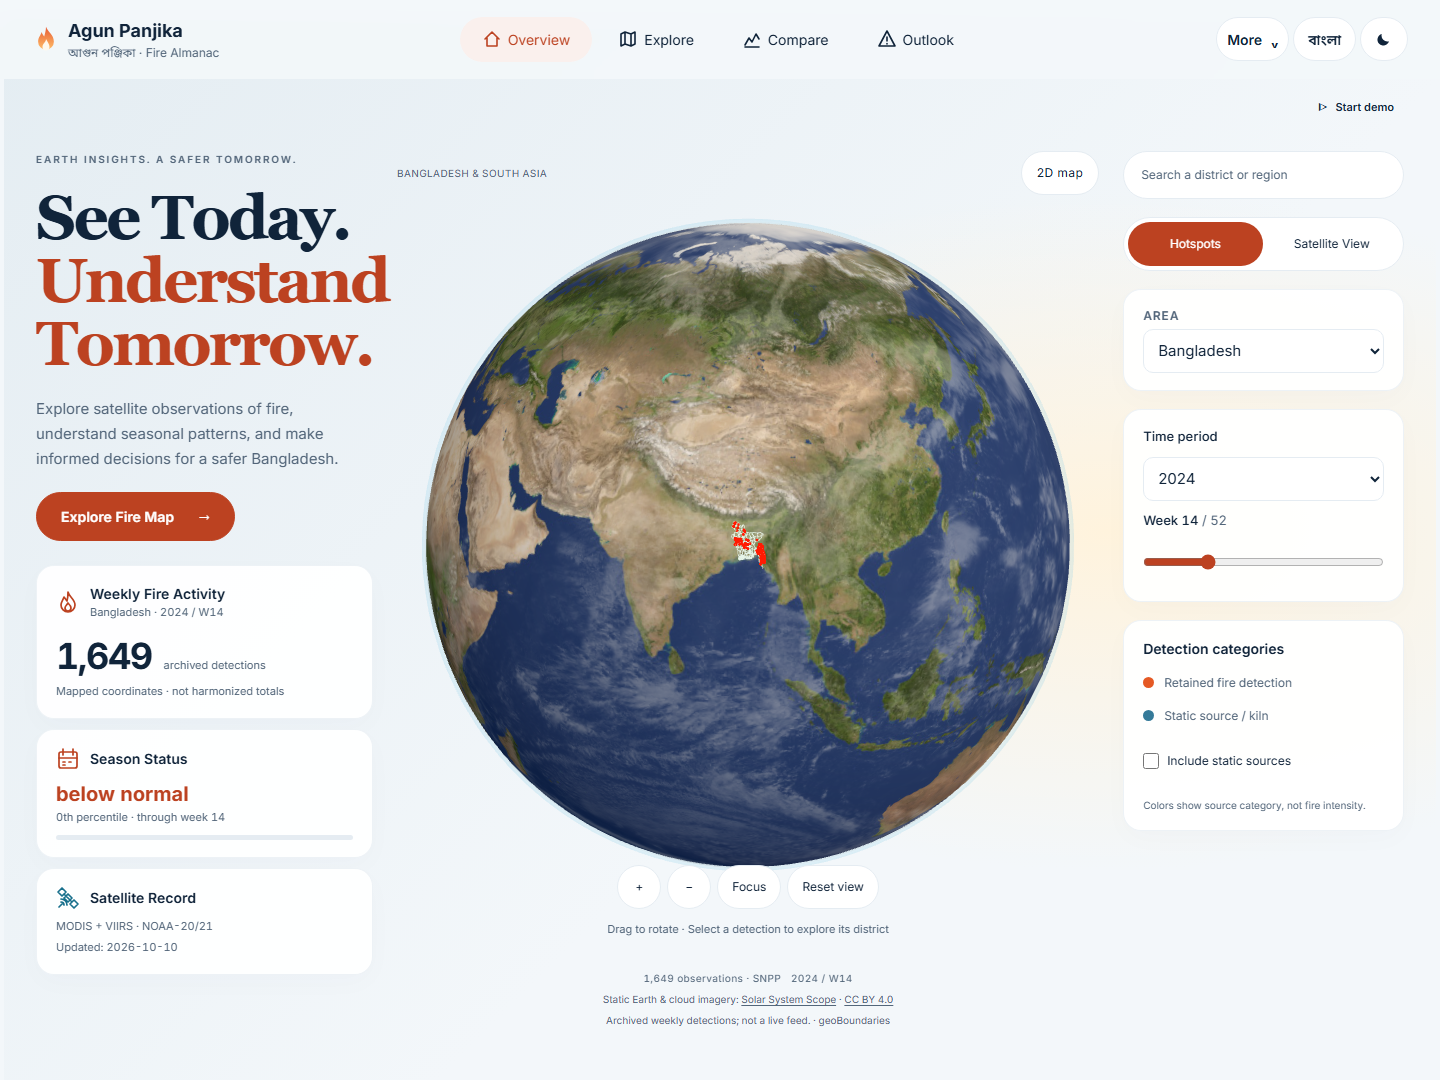
\includegraphics[width=\linewidth]{../review/screenshots/home-desktop.png}
\vspace{4mm}
{\sffamily\bfseries Team KUETaguns}\par
Khulna University of Engineering \& Technology (KUET), Bangladesh\par
\vfill
\begin{minipage}[t]{.6\linewidth}\small
\textbf{Proposal for mentor discussion}\par
Prepared \ReviewDate. Extensions are future work; an award or globally valid accuracy is not guaranteed.
\end{minipage}\hfill
\begin{minipage}[t]{.34\linewidth}\small\raggedleft
\href{\Repo}{Source repository}\par
\RepoLink{docs/PROJECT_BRIEF.md}{Companion project brief}\par
\RepoLink{docs/GLOBAL_EXTENSION_PLAN.md}{Detailed Markdown plan}
\end{minipage}

\ReportPage{Decision, scope and proposed contribution}{sec:scope}
\begin{keypoint}{Recommended direction}
Make sensor comparability inspectable: a user chooses an evaluated area, compares its fire history across sensors, sees uncertainty and data sufficiency, and exports a dated evidence brief.
\end{keypoint}

The current application already contains calendars, maps, a textured Earth, bilingual reports, guided storytelling and experimental outlooks. The strongest next contribution is better scientific and practical evidence for the central calendar, rather than more screens or visual effects.

\subsection{What exists and what is proposed}
\begin{table}[H]\small
\begin{tabularx}{\linewidth}{@{}L{33mm}YY@{}}
\toprule
\textbf{Area} & \textbf{Current foundation} & \textbf{Proposed extension}\\\midrule
Geography &Bangladesh, five regions, 64 districts; a Nepal configuration &Two or three independently evaluated, contrasting area packages.\\
Scientific comparison &Raw/factor/harmonized series and internal validation &Locked holdout, fold-local preprocessing/calibration and complete failure reporting.\\
Sensor explanation &Sensors screen and successor diagnostics &Held-out sensor-transition experiment linked to the calendar.\\
Interpretation &Uncertainty/source labels, bilingual reports &Visible data-sufficiency state and portable dated evidence brief.\\
Practical value &Intended users; an uncompleted study protocol &Recorded practitioner/comprehension pilot and revisions based on observed errors.\\\bottomrule
\end{tabularx}
\caption{Current capabilities are distinct from future deliverables. Country configuration alone does not establish transfer performance.}
\end{table}

\subsection{Three research questions}
\begin{enumerate}
\item Does the reconstruction improve on strong simple baselines under independent temporal and geographic evaluation?
\item Are uncertainty and data-sufficiency statements reliable across activity levels, sensor changes and missing-data conditions?
\item Can intended users correctly interpret a season's status and limitations, and use the brief in a real workflow?
\end{enumerate}

\subsection{Scope boundary}
The first extension should use \textbf{supported, evaluated areas}. Arbitrary polygon computation and operational warning integration follow only after suitable architecture and validation. No worldwide accuracy, agency adoption, smoke-arrival prediction or prevention benefit should be inferred from a global-looking map.

\SourceNote{The proposal builds on the reviewed implementation and saved results. Its purpose is stronger validity, relevance and usefulness, not a promise of competition selection.}

\ReportPage{Work package 1: scientific independence}{sec:science}
\subsection{Lock the evaluation before extending the claims}
The existing Bangladesh benchmark reports a 25.25\% weekly-MAE improvement over a fitted factor. That result is internal. Strengthen the protocol before adding countries or repeating a broader accuracy claim.

\begin{enumerate}
\item \textbf{Reserve an untouched assessment.} Agree on temporal/geographic splits with a domain reviewer. Lock features, model weights, tuning and reporting rules before evaluating the final holdout.
\item \textbf{Fit learned steps within the split.} Static-source decisions, reconstruction/preprocessing and calibration must use permitted training data only. Evaluation-year exclusion must apply to every model fit used to generate calibration residuals, not only to the residual list.
\item \textbf{Separate reconstruction from forecasting.} The current reconstruction uses next-week MODIS counts. Define retrospective availability explicitly; prospective evaluation must respect issue-time source latency and use archived weather forecasts.
\item \textbf{Retain strong baselines.} Compare fixed 4.4$\times$, fold-fitted and monthly factors, negative binomial and bagged LightGBM with the ensemble. Publish ablations and the conditions where a simpler model is adequate.
\end{enumerate}

\subsection{Evaluate uncertainty and failure modes}
Report national/regional weekly MAE, off-season error, annual-total error, interval coverage and width. Include weak years, sparse areas and failures; average improvements alone are insufficient. Forecast intervals need separate calibration, and the observed-future-FWI experiment remains an optimistic sensitivity test.

Exercise sensor handover across main, district/local, neighbour and point products. Test real zeros, missing coverage, one/both successor sensors, month boundaries and a deliberately nonidentity correction. The current identity selection can conceal divergent product behavior.

For static-source filtering, lock the heuristic and inspect a new blind sample. Record positive, negative and uncertain labels, sampling uncertainty and wrongly removed vegetation fires. The tuned final 16/20 positive sample is not an independent precision/recall assessment.

\begin{keypoint}{Exit condition}
A reviewer-agreed protocol, versioned split/input manifest and reproducible result table exist. Final results include failures and all stated baselines; uncertainty calibration is independently assessed. Passing thresholds are set before the final evaluation, not chosen after seeing its results.
\end{keypoint}

\SourceNote{Detailed source concerns: \RepoLink{docs/SCIENTIFIC_REVIEW.md}{scientific review}. Protocol and new experiments are proposed work; this report does not re-estimate the existing scores.}

\ReportPage{Work package 2: evaluated areas and transitions}{sec:areas}
\subsection{A bounded global demonstration}
Keep Bangladesh as the reference case, reproduce the Nepal example, and select a third setting with a domain reviewer because its fire seasonality, land cover or static-source mix tests a different assumption. A case is successful only if it meets predeclared criteria; unsuccessful cases remain visible as experimental or unsupported.

Each case should publish its boundary/version, sensor coverage and overlap, training/evaluation cutoffs, baselines, the same metric definitions, interval diagnostics and failure analysis. Any independent burned-area/local evidence is described as a cross-check of its own observable. Fresh reproducible results are needed before using an older Nepal claim in a new submission.

\begin{figure}[H]\centering
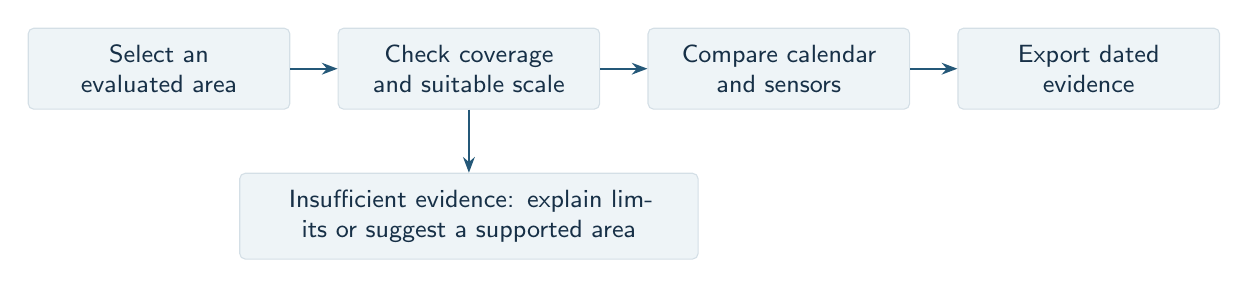
\begin{tikzpicture}[node distance=6mm]
\node[box,text width=29mm] (a) {Select an\\evaluated area};
\node[box,text width=29mm,right=6mm of a] (b) {Check coverage\\and suitable scale};
\node[box,text width=29mm,right=6mm of b] (c) {Compare calendar\\and sensors};
\node[box,text width=29mm,right=6mm of c] (d) {Export dated\\evidence};
\node[box,text width=54mm,below=8mm of b] (n) {Insufficient evidence: explain limits or suggest a supported area};
\draw[arrow](a)--(b);\draw[arrow](b)--(c);
\draw[arrow](c)--(d);\draw[arrow](b)--(n);
\end{tikzpicture}
\caption{Proposed interaction. Abstention is part of the scientific contract, rather than a missing feature disguised as zero activity.}
\end{figure}

\subsection{Area packages before arbitrary polygons}
The current model learns region-week aggregates. A polygon-drawing control cannot create a calibrated history by filtering the existing point export: required features, suitable overlap and scale-dependent evaluation are missing. Begin with prebuilt area packages that the static app can select.

An area specification should contain geometry/boundary version, time window, source sensors, coverage thresholds and data/model version. The pipeline produces a reproducible evaluated package, preserving observed/estimated provenance. Later custom areas need asynchronous/server computation or a validated spatial aggregation method; keep FIRMS credentials on the pipeline/server side.

\subsection{Make a sensor transition inspectable}
Extend the existing Sensors screen with one area, period and transition date. Display raw observations, naive stitching, a fitted-factor result and harmonized history on comparable axes. In an overlap experiment, withhold the reference sensor for a period, reconstruct it and reveal the held-out observations. Expose the training/evaluation periods.

The accompanying evidence panel and export should retain area, source, completeness, model version, error, interval and data-through date. For periods without a reference sensor, label reconstruction and uncertainty explicitly.

\SourceNote{Exit condition: an added area is reproducible and either meets its declared requirements or visibly abstains. A user can distinguish the sensor artifact, the supported comparison and the estimated period.}

\ReportPage{Work package 3: users, access and release}{sec:users}
\subsection{Test comprehension and workflow fit}
Use the existing five-person protocol as a pilot. Include at least one relevant practitioner if feasible and arrange native Bangla/CHT terminology review. Intended users and personas do not substitute for participants or evidence of adoption.

Ask each participant to choose an area, judge whether a selected season is unusual, identify estimated periods/uncertainty, and share a report that preserves its caveats. Record correctness, time, language, device and the participant's explanation; revise the interface from observed misunderstandings.

\begin{table}[H]\small
\begin{tabularx}{\linewidth}{@{}L{35mm}Y@{}}
\toprule
\textbf{Pilot task} & \textbf{Proposed acceptance evidence}\\\midrule
Interpret a season &At least four of five correct answers; median time below ten seconds, following the repository's pilot targets.\\
Understand provenance &At least four of five can find the data date and explain estimated/observed periods and the interval.\\
Recognize insufficient data &Participants distinguish missing/sparse coverage from low activity and explain the abstention.\\
Fit an actual workflow &A practitioner records the decision, objections and evidence needed; review is not agency adoption.\\
Use it on a phone/offline &Keyboard/table access and readable small-screen report; cached resources remain usable with disclosed limits.\\\bottomrule
\end{tabularx}
\caption{Pilot criteria are proposed, not achieved outcomes. A larger study is needed for population-wide usability or impact claims.}
\end{table}

Measure the existing sub-three-second mobile LCP target on a declared device/throttling setup. Local desktop timings do not establish that target. Do not infer fires prevented, lives saved or operational warning benefit from a small comprehension study.

\subsection{Make the result reliably reviewable}
\begin{itemize}
\item Diagnose the hosted pipeline failure, publish a working demo URL and verify refresh/build/deploy. A local pass does not establish hosted operation.
\item Expose source completeness, version, data-through date and stale status. Expire or clearly label old forecast products; missing acquisition chunks must not silently appear as zero activity.
\item Synchronize Method text, translations, citations, README and video claims with one result table. The current in-app 50/50 and 2012--2024 wording differs from the 30/70, 2012--2025 model/export.
\item Review dependency advisories separately, choose an explicit software license, and preserve data/imagery credits and required AI-use disclosures.
\end{itemize}

\SourceNote{Exit condition: a dated public demo works, a pilot is completed, misunderstandings produce documented revisions, and a portable evidence brief preserves the scientific limits.}

\ReportPage{Milestones, dependencies and risks}{sec:milestones}
The sequence below is dependency-based. It is not a set of competition deadlines or an existing team commitment. Assign owners and timing after the mentor helps narrow scope.

\begin{table}[H]\small
\begin{tabularx}{\linewidth}{@{}L{27mm}YY@{}}
\toprule
\textbf{Milestone} & \textbf{Deliverable} & \textbf{Exit condition}\\\midrule
A. Baseline &Aligned method/result note, frozen snapshot and public demo &Link works; freshness/version visible; local checks and hosted refresh pass.\\
B. Protocol &Agreed protocol and reproducible benchmark &Splits/calibration reviewed; final scores and failures reported.\\
C. Transfer &Additional evaluated area and transition comparison &Reproducible package with baseline/error/coverage evidence and support limits.\\
D. Pilot &Completed pilot and revised user journey &Task/uncertainty comprehension recorded; revisions trace to observed errors.\\
E. Package &Short demo/slides, description, evidence links and credits &Applicable rules confirmed; public links work; numerical claims trace to artifacts.\\\bottomrule
\end{tabularx}
\caption{Complete one bounded deliverable before broadening geography, architecture or operational claims.}
\end{table}

\subsection{Research and engineering risks}
\begin{table}[H]\small
\begin{tabularx}{\linewidth}{@{}L{42mm}Y@{}}
\toprule
\textbf{Risk} & \textbf{Response in the plan}\\\midrule
Transfer fails or requires recalibration &Publish the failure and local adjustments; limit supported cases rather than claim global validity.\\
Coverage/calibration is unreliable &Set requirements with a reviewer, show interval width and abstain on unsupported conditions.\\
Custom areas exceed the static architecture &Deliver evaluated area packages first; select new processing infrastructure from measured needs.\\
Feature growth outpaces evidence &Prioritize the benchmark, one transition workflow and one user journey.\\
Rules or permitted edits are uncertain &Confirm with organizers before treating later work as competition-evaluable.\\\bottomrule
\end{tabularx}
\end{table}

\begin{keypoint}{Smallest credible next deliverable}
One reproducible, independently assessed comparison beyond the baseline, linked to a working calendar and a user who can explain its uncertainty. This can be a stronger Bangladesh case or a validated transfer case, depending on the mentor's advice.
\end{keypoint}

\ReportPage{Submission story and mentor decisions}{sec:decisions}
\subsection{A focused demonstration}
Show the sensor discontinuity, reveal the comparable calendar and uncertainty, demonstrate one evaluated transfer case, and close with the user's decision. Use only metrics that can be explained and reproduced. The current 2:42 video remains useful background; a separate short global demonstration may be necessary.

The supplied Bangladesh guide distinguishes local 240-second presentations from a global under-30-second video or seven-slide alternative. It calls for public links, English presentation/subtitles, source credits and AI-use disclosure. It contains conflicting cutoffs and is not independently established as final global policy. Confirm format, deadlines and permitted edits with the Local Lead and final official guidance.

\subsection{What a stronger submission would show}
\begin{table}[H]\small
\begin{tabularx}{\linewidth}{@{}L{31mm}Y@{}}
\toprule
\textbf{Review lens} & \textbf{Inspectable evidence}\\\midrule
Scientific validity &Independent evaluation, baseline comparisons, calibrated uncertainty and complete failure reporting.\\
Challenge relevance &A comparable history and calendar through an actual or held-out sensor transition.\\
Practical impact &Recorded interpretation tasks and a practitioner's documented workflow need.\\
Creativity &An understandable transition reveal and a useful insufficient-evidence state.\\
Presentation &Working public materials, readable dated brief, focused demo and source attribution.\\\bottomrule
\end{tabularx}
\caption{Planning lenses, not a confirmed global scoring formula or a prediction of an award.}
\end{table}

\subsection{Four decisions to take to the mentor}
\begin{enumerate}
\item What independent evaluation is necessary for the central harmonization claim?
\item Is the next priority a stronger Bangladesh pilot or an evaluated additional-country case?
\item Which user decision, practitioner and domain reviewer should shape the prototype?
\item How should the contribution be positioned against existing sensor-fusion work?
\end{enumerate}

\subsection{Supporting material}
\begin{itemize}\small
\item \RepoLink{docs/PROJECT_BRIEF.md}{Project brief}, \RepoLink{docs/SCIENTIFIC_REVIEW.md}{scientific review}, \RepoLink{docs/VERIFICATION.md}{verification record}, \RepoLink{docs/Agun\%20Panjika\%20\%E2\%80\%94\%20User\%20Test\%20Protocol.md}{user-test protocol} and \RepoLink{docs/SOURCES_AND_SUBMISSION.md}{credits/submission notes}.
\item \href{https://docs.google.com/document/d/1mSOxplyht5kii8GcCnFaGA-vMHIAVypjl4N6PobnaYQ/edit}{Supplied 2026 Bangladesh Participants Guide}; \href{https://www.spaceappschallenge.org/2026/}{official Space Apps site}; \href{https://youtu.be/9FMIzcXhqB4}{team video}.
\end{itemize}
\SourceNote{NotebookLM required login and the supplied Claude artifact content was inaccessible during the review; neither was used to infer rules. The detailed Markdown plan retains the fuller evidence and source-access notes.}
\end{document}
